%%%%%%%%%%%%%%%%%%%%%%%%%%%%%%%%%%%%%%%%%

%----------------------------------------------------------------------------------------
%	PACKAGES AND OTHER DOCUMENT CONFIGURATIONS
%----------------------------------------------------------------------------------------

\documentclass{article}

\input{C:/Code/TexStudio/templates/structure.tex} % Include the file specifying the document structure and custom commands

%----------------------------------------------------------------------------------------
%	ASSIGNMENT INFORMATION
%----------------------------------------------------------------------------------------

\title{Assignment \#5} 
% Title of the assignment

\author{Name:Cao Mingming \indent \indent ID:2018311770\\ \texttt{cmm18@mails.tsinghua.edu.cn}} 
% Author name and email address

\date{Tsinghua University --- \today} 
% University, school and/or department name(s) and a date


\begin{document}
\maketitle % Print the title

\section{Problem 1} % Unnumbered section

Derive Eq. 2.64 and Eq. 2.65 in the main textbook.
\section*{Solution 1}
Assumed that the q parameter at the left of the lens is $q_1$ and the beam wasit at the right side is $q_2$, as is known in the figre 1.
\begin{figure}[h]
    \centering
    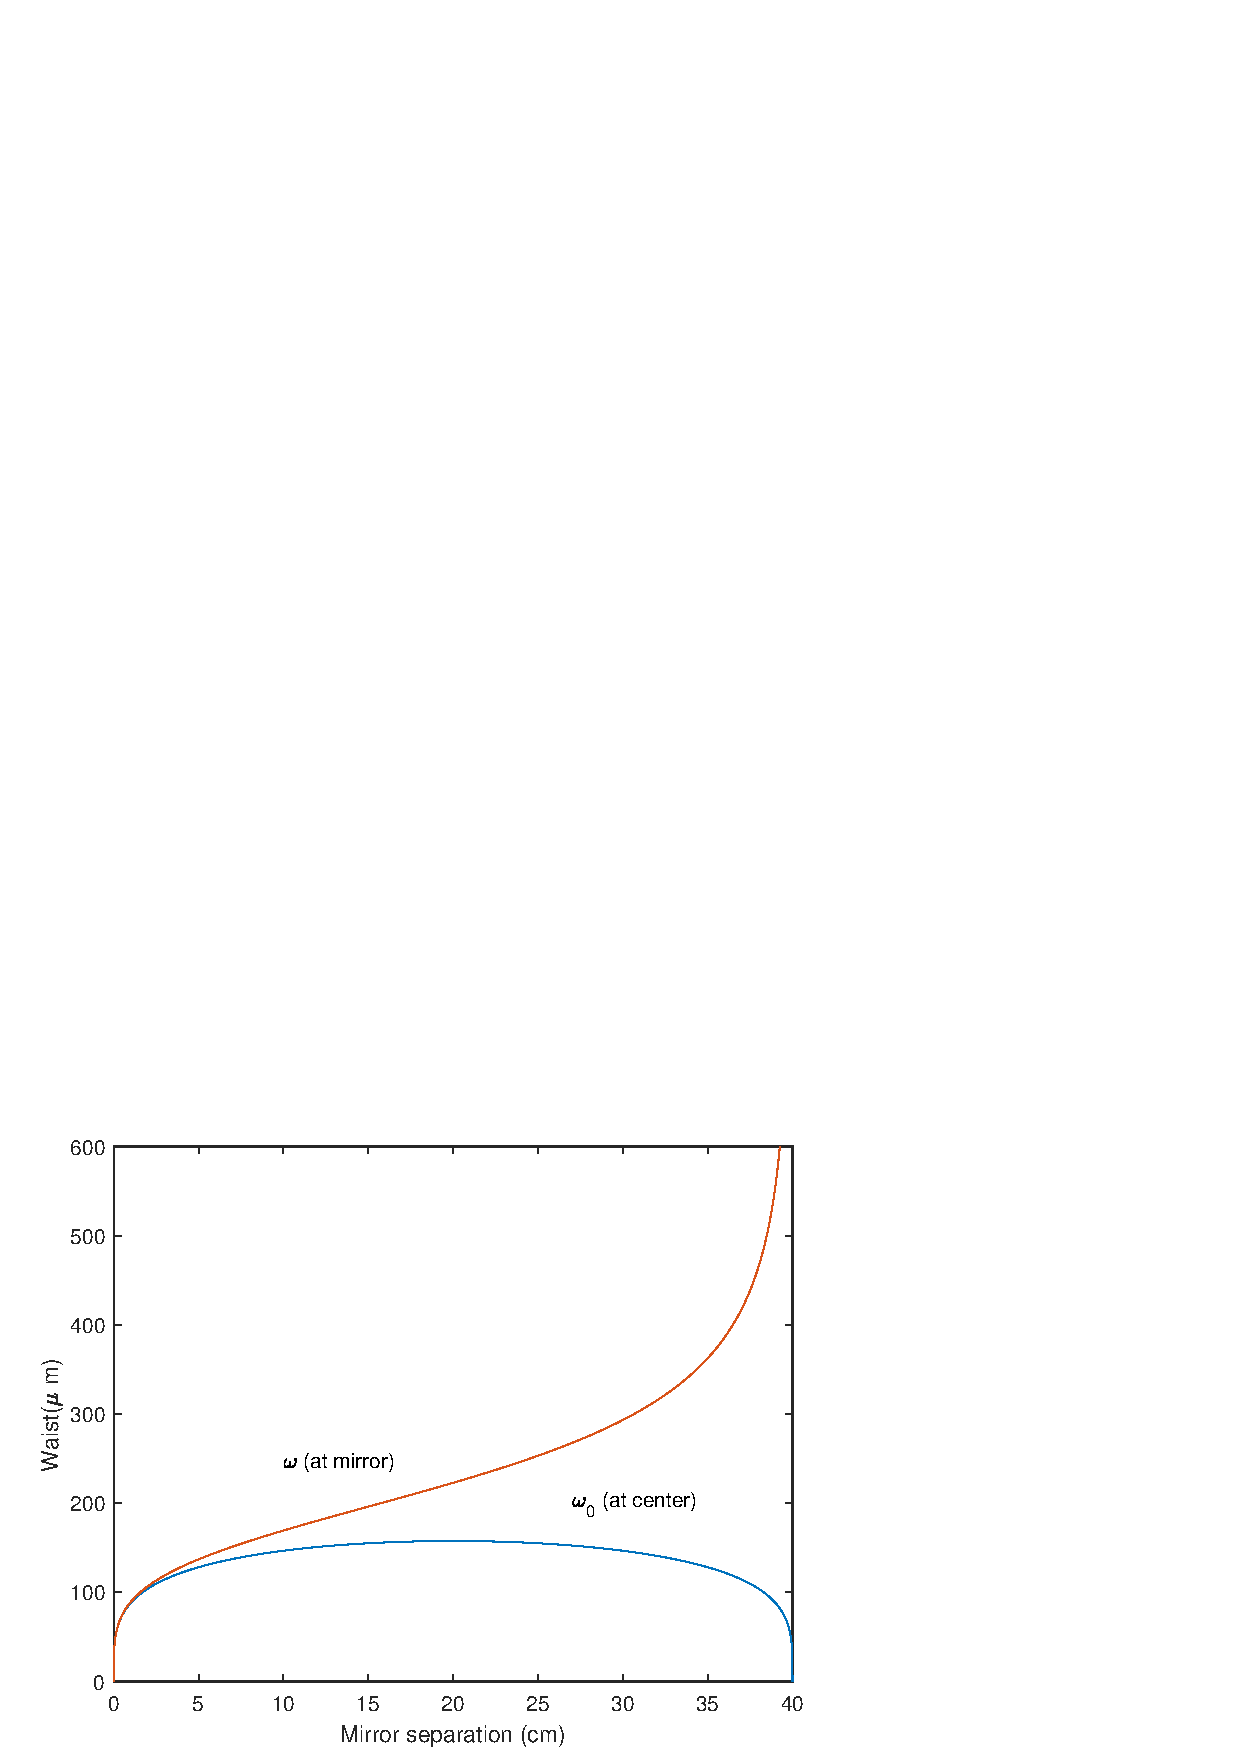
\includegraphics[width=9cm]{f1.png}
    \caption{Mode mathcing}
    \label{fig1}
\end{figure}
The ABCD matrix of lens is,
\begin{equation}\label{eq1}
	M=
    \begin{pmatrix}
         1 & 0 \\
         -\frac{1}{f}  & 1
    \end{pmatrix}
\end{equation}

Therefore we could get,
\begin{equation}\label{eq2}
    \begin{aligned}
        q_1&=d_1+i\frac{n\pi\omega_1^2}{\lambda}
        \\ 
        \\
        q_2&=\frac{Aq_1+B}{Cq_1+D}+d_2\\
        \\
        &=\frac{fq_1}{f-q_1}+d_2
        \\
        \\
        &=\frac{f(d_1+iZ_{R1})(f-d_1+iZ_{R1})}{(f-d_1)^2+Z_{R1}^2}+d_2
    \end{aligned}
\end{equation}
$q_2$ is the q paramter at the right beam wasit therefore we know that,

\begin{equation}\label{eq3}
        \begin{aligned}
        q_2&=iZ_{R2} \\
        \\ 
        &=\frac{n\pi\omega_{2}^2}{\lambda}
        \end{aligned}
\end{equation}
which is a pure imaginary number.
Compare equaiton 2 with euqaiton 3 we can get that,

\begin{equation}
    i\frac{f^{2} Z_{R1}}{(f-d_{1})^2+Z_{R1}^2}+\frac{f[d_1(f-d_1)^2-Z_{R1}^2+d_2(f-d_1)^2]}{(f-d_1)^2+Z_{R1}^2}+d_2=iZ_{R2}
\end{equation}
which indicate that,
\begin{equation}\label{eq5}
	\begin{array}{l}
	\frac{f^{2} Z_{R1}}{(f-d_{1})^2+Z_{R1}^2}=Z_{R2}\\
	\\
	\frac{f[d_1(f-d_1)^2-Z_{R1}^2+d_2(f-d_1)^2]}{(f-d_1)^2+Z_{R1}^2}+d_2=0
	\end{array}
\end{equation}
Solving above equation we could get,
\begin{equation}
    \begin{aligned}
    d_1&=f\pm\frac{\omega_1}{\omega_2}\sqrt{f^2-f_{0}^2} \\
    \\
    d_2&=f\pm\frac{\omega_2}{\omega_1}\sqrt{f^2-f_{0}^2}
    \end{aligned}
\end{equation}



\section{Problem 2}
The mode-matching techniques for standing wave cavities described in the text
did not take account of the refractive power of the input mirror which acts like
a weak negative lens. Assume that one has an approximately confocal cavity
with mirror separation $d$. Approximately how far is the apparent waist position
shifted by refraction from the input mirror? (Treat the input mirror as a thin
plano-concave lens with refractive index n.) Assume $n = 1.5$ and determine the
actual shift in terms of $d$.
\section*{Solution}
Suppose the radius of the cavity are $R1$ and $R_2$, due to that it is a confocal cavity we know that,
\begin{equation}\label{key}
	R_1=R_2=d
\end{equation}
Using the equation of lens maker, the focal length of the plano-concave lens is $f$,
\begin{equation}\label{key}
	f=(\frac{n2}{n_1}-1)(\frac{1}{R_1}+\frac{1}{R_2})
\end{equation}
Substitute $n_1=1, \quad n_2=1.5, \quad R_1=d, \quad R_2=\infty$ into the above equation we can get,
$$f=2d$$
\begin{figure}[h]
	\centering
	\includegraphics[width=0.7\linewidth]{f21}
\end{figure}
Therefore the ABCD matrix of the plano-concave lens is $M_1$,
$$
M_1=
\begin{pmatrix}
1 & 0\\
\frac{1}{2d} & 1
\end{pmatrix}
$$
Assume that the q parameter at the left mirror is $q_1=-\frac{d}{2}+iZ_R$ where,
$$
Z_R=\frac{n\pi\omega_0^2}{\lambda}=\frac{d}{2}
$$
using ABCD matrix of the plano-concave lens we can get,
\begin{equation}\label{key}
	q_2=\frac{Aq_1+B}{Cq_1+D}
\end{equation} 
Substitute $M_1$ and $q_1$ into equation 9 we can get,
\begin{equation}\label{key}
		q_2=\frac{-6d^3+8dZ_R^2+(4d^2Z_R+12d^2Z_R)i}{9d^2+4Z_R^2}
\end{equation}
Therefore the distance of beam waist from the left mirror is,
\begin{equation}\label{key}
	d_1=\frac{-6d^3+8dZ_R^2}{9d^2+4Z_R^2}=-\frac{2}{5}d
\end{equation}
Therefore the beam waist has a shift of $\frac{d}{10}$ to the left.
\section{Problem 3}

\begin{figure}[ht]
	\centering
	\includegraphics[width=1.1\linewidth]{f3}
\end{figure}

\section*{Solution}
\subsection{PART I}
\begin{figure}[h]
	\centering
	\includegraphics[width=0.7\linewidth]{f2}
\end{figure}
The ABCD mtrix of the lens is,
\begin{equation}\label{key}
	\begin{aligned}
			M_2&=
		\begin{pmatrix}
		1 & 0\\
		-\frac{1}{f_2} & 1
		\end{pmatrix}
		\begin{pmatrix}
		1 & d\\
		0 & 1
		\end{pmatrix}
		\begin{pmatrix}
		1 & 0\\
		-\frac{1}{f_1} & 1
		\end{pmatrix}\\
		\\
		&=\begin{pmatrix}
		1-\frac{d}{f_1} & d\\
		-\frac{1}{f_1}--\frac{1}{f_2}+\frac{d}{f_1f_2} & 1-\frac{d}{f_2}
		\end{pmatrix}
	\end{aligned}
\end{equation}
Assume that the q parameter at lens $f_1$ is $q_1=iZ_1$, where $Z_1=\frac{n\pi\omega_1^2}{\lambda}$, therefore we could get the q parameter at the lens $f_2$ as,
\begin{equation}\label{key}
	\begin{aligned}
		q_2&=\frac{Aq_1+B}{Cq_1+D}
		\\
		\\
		&=\frac{BD+ACZ_1^2}{B^2+A^2Z_1^2}+i\frac{(BC-AD)Z_1}{B^2+A^2Z_1^2}
	\end{aligned}
\end{equation}
$q_2$ is also a part of the beam of the cavity, therefore starting from the beam wasit of the cavity we can write $q_2$ as,
\begin{equation}\label{key}
	q_2=-d_0+iZ_0
\end{equation}
where $Z_0=\frac{n\pi\omega_0^2}{\lambda}$. Comparing equation 13 with equation 14 we could derive that,
\begin{equation}\label{key}
	\begin{array}{l}
		Z_0=Im(q_2)=\frac{(BC-AD)Z_1}{B^2+A^2Z_1^2}\\
		\\
		d_0=-Re(q_2)=-\frac{BD+ACZ_1^2}{B^2+A^2Z_1^2}
	\end{array}
\end{equation}
Substitute the element in $M_2$ into the above equation we can simplify equation as ,
\begin{equation}\label{key}
	Z_0[(f_1f_2-f_1d)^2+Z_1^2(f_1+f_2-d)^2]=f_1^2f_2^2Z_1
\end{equation}
Using mathematics to solve equation 17 we can get d as,
\begin{equation}\label{key}
	d=f_1+f_2+f_1^2\frac{f_1\pm\sqrt{-Z_1^2+\frac{Z_1^3}{Z_0}(\frac{f_2^2}{f_1^2})+\frac{Z_1}{Z_0}f_2^2}}{Z_1^2+f_1^2}
\end{equation}
Substitue  $\frac{f_1}{f_2}=\frac{\omega_1}{\omega_2}=\frac{1}{\sqrt{1+(d_0\//Z_0)^2}}\frac{\omega_1}{\omega_0}$ into eqaution 17 we can get,
\begin{equation}\label{key}
    \begin{aligned}
     d&=(f_1+f_2)+f_1^2\frac{f_1\pm\sqrt{(\frac{d_0}{Z_0})^2Z_1^2+\frac{Z_1}{Z_0}f_2^2}}{Z_1^2+f_1^2}\\
     \\
     &=(f_1+f_2)+f_1^2\frac{f_1\pm\sqrt{d_0^2Z_1^2+f_2^2}}{Z_0(Z_1^2+f_1^2)}
    \end{aligned}
\end{equation}

Therefore $\Delta d=f_1^2\frac{f_1\pm\sqrt{d_0^2Z_1^2+f_2^2}}{Z_0(Z_1^2+f_1^2)}$ and we need to move slightly more than $f_1+f_2$ to make the beam waist at the center of cavity.
\subsection{Part II}
However, we note that under the condition
$$
	\frac{f_1}{f_2}=\frac{\omega_1}{\omega_0}=\sqrt{\frac{Z_1}{Z_0}}
$$
equation 17 can be simplified as,
\begin{equation}\label{key}
	q_2=(f_1+f_2)+\frac{f_1^2(f_1\pm f_1)}{f_1^2+Z_1^2}
\end{equation}
which indicates that,
\begin{equation}\label{key}
	d=f_1+f_2 \quad or\quad  f_1+f_2+\frac{2f_1^3}{f_1^2+Z_1^2}
\end{equation}
therefore there exists a strict analytic solution $d=f_1+f_2$ under such condition.
\subsubsection{1)}
Due to the radius of the confocal cavity is $R$ therefore we could get $d=R=10cm$, $Z_0=\frac{d}{2}=5cm$, $Z_1=3.14m$, $\omega_0=\sqrt{\frac{\lambda d}{2n\pi}}\approx 0.178mm(n=1)$. Choose $d_0=R=10cm$ and   $\omega_2=\sqrt{2}\omega_0=0.252mm$ and set
\begin{equation}\label{key}
	\frac{f_1}{f_2}=\frac{\omega_1}{\omega_0}\approx 4
\end{equation}
Hence we choose $f_1=40mm$, $f_2=10mm$ and $d=f_1+f_2=50mm$ and $\Delta d=\pm1mm$

\subsubsection{2)}
Frome the question we know that $\omega_0=20\mu m$, $\omega_1=1mm$ therefore we could get
\begin{equation}\label{key}
	\begin{array}{l}
	Z_0=\frac{n\pi\omega_0^2}{\lambda}=2.4mm\quad (n=1)\\
	\\
	Z_1=\frac{n\pi\omega_0^2}{\lambda}=5.9m\\
	\\
	setting d_0=10*Z_0=24mm\\
	\\
	\omega_2=\omega_0*\sqrt{1+(d_0\//z_0)^2}=201\mu m\\
	\\
	\frac{f_1}{f_2}=\frac{\omega_1}{\omega_2}=4.97
	\end{array}
\end{equation}
Set $d_0=10*Z_0=24mm$ and $f_2=10mm$ we could get $f_1\approx50mm$, $d=f_1+f_2=60mm$ and $\Delta d=-4.1mm \quad or \quad  4.3 mm$
\end{document}